\section{Архитектура библиотеки}

В данной секции представлена архитектура разработанной библиотеки, описание основных компонентов и модулей, а также показана последовательность обработки операций и концепция организации вычислений на GPU.

Структура библиотеки и ее конченная функциональность в основном определяется следующими высокоуровневыми требованиями, которые продиктованы как конечными вычислительными задачами на GPGPU, так и наличием существующей инфраструктуры для осуществления экспериментов~\cite{net:cfpq_py_algo}.

\begin{itemize}[noitemsep,topsep=0pt,parsep=0pt,partopsep=0pt]
    \item \textit{Поддержка вычислений на Cuda-устройстве.} В качестве GPGPU технологии необходимо использовать Nvidia Cuda, поскольку в библиотеке необходимо повторно использовать уже существующий код для работы с разреженными матрицами из исследования Арсения Терехова и др.~\cite{inproceedings:cfqp_matrix_with_single_source}.
    \item \textit{Поддержка вычислений на CPU.} Пользователь сможет запустить вычисления с использованием библиотеки, даже если его компьютер не оснащен Cuda-устройством.
    \item \textit{C-совместимый API для работы с библиотекой.} Примитивы и операции библиотеки доступны в среде с неуправляемыми ресурсами для вызова библиотечных функций без накладных расходов, что критически важно для обработки больших массивов данных.
    \item \textit{Python-пакет для работы с библиотекой.} Примитивы и операции будут доступны в высокоуровневой среде с управляемыми ресурсами, что снизит порог вхождения и упростит процесс прототипирования алгоритмов.
    \item \textit{Поддержка логирования, функций для отладки конечных пользовательских алгоритмов.} Конечные пользовательские алгоритмы могут иметь нетривиальную структуру, поэтому требуются встроенные в библиотеку инструменты для отладки.
\end{itemize}

\begin{figure}[h]
    \centering
    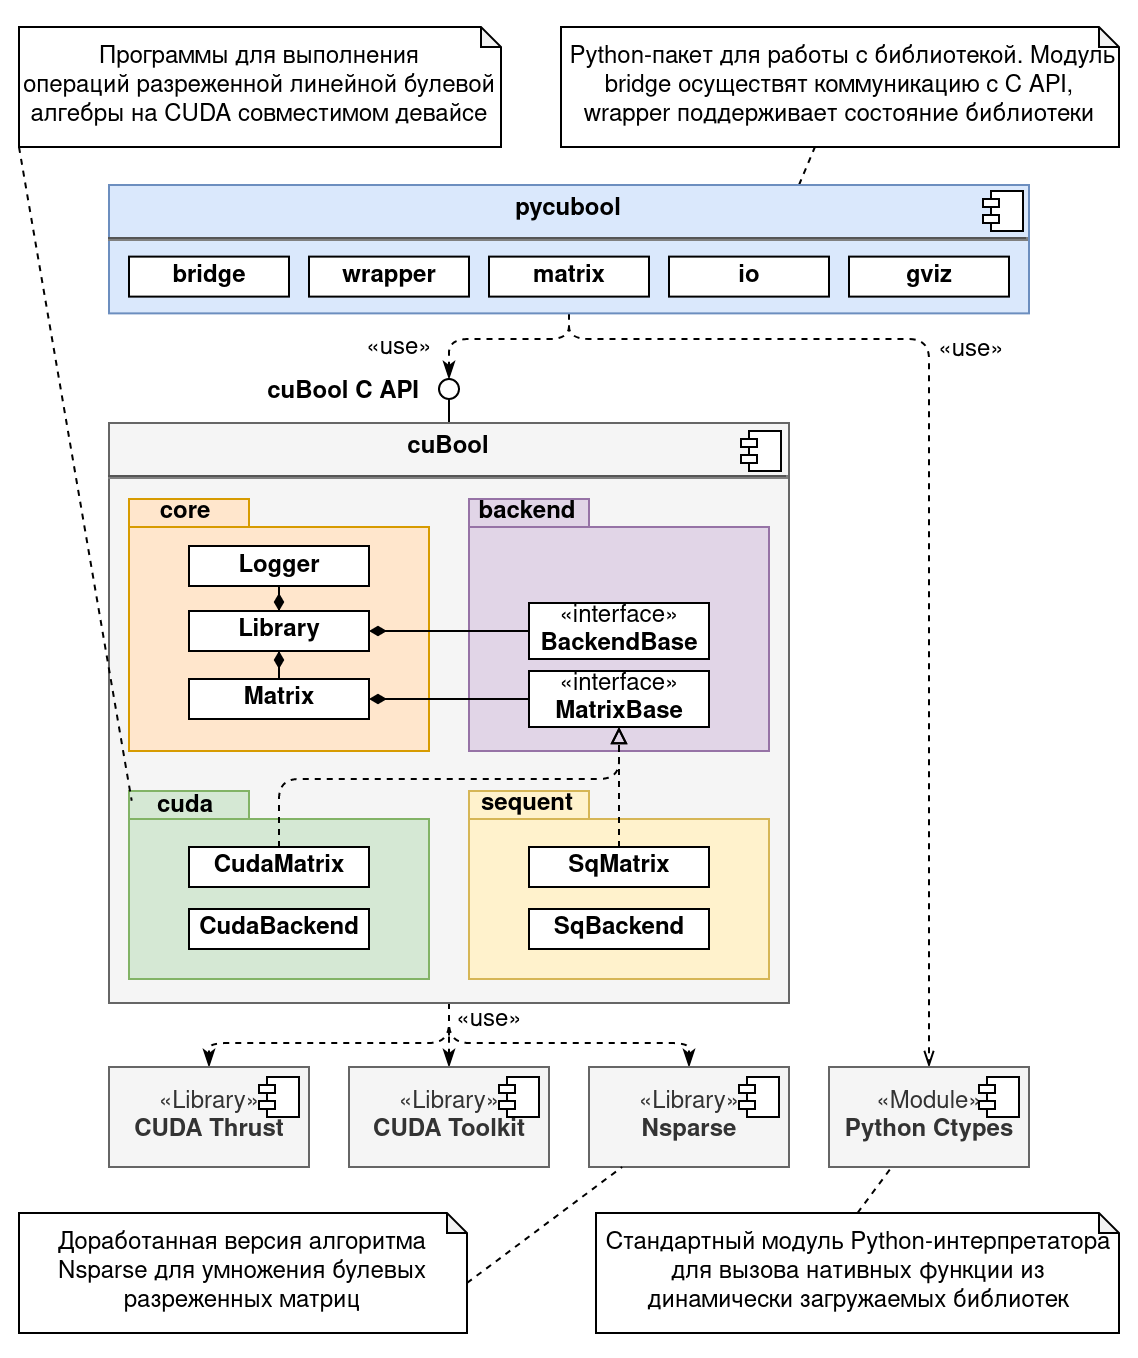
\includegraphics[width=0.8\textwidth]{images/library_architecture.png}
    \caption{Архитектура разработанной библиотеки}
    \label{fig:cubool_architecture}
\end{figure}

\subsection{Компоненты библиотеки}

Далее предлагается детально рассмотреть основные компоненты разработанной библиотеки \textbf{cuBool}.
Библиотека имеет модульную структуру. 
Интерфейс представлен C-совместимым API, что отвечает требованиям проекта.
Также библиотека предоставляет Python-пакет \textbf{pycubool}.
Архитектура библиотеки представлена на рис.~\ref{fig:cubool_architecture}.
Сторонние зависимости проекта на рисунке обозначены белым цветом и находятся на нижнем уровне диаграммы. 
Далее представлено детальное описание основных компонент библиотеки.

\subsubsection*{Core}

Класс \textbf{Library} поддерживает глобальное состояние библиотеки, осуществляет конфигурацию и инициализацию, выбор конкретного вычислительного модуля, первичную валидацию вызовов функций и входных данных пользователя, 
а также хранит все созданные пользователем объекты. 

Класс \textbf{Matrix} является proxy-классом, который осуществляет доступ к операциям конкретного вычислительного модуля, выбранного пользователем на этапе инициализации всей библиотеки.
Данный подход позволяет не только динамически выбирать платформу вычислений, 
но и позволяет осуществлять дополнительную обработку ошибок, 
а также поддерживать дополнительные операции над матрицами.

Класс \textbf{Logger} осуществляет логирование в выбранный пользователем текстовый файл в процессе использования функций библиотеки, а также позволяет профилировать операции и также сохранять время их выполнения в текстовом виде.

\subsubsection*{Backend}

Интерфейс \textbf{MatrixBase} предоставляет набор основных функций и операций, которые каждый вычислительный модуль должен реализовывать, чтобы предоставляемые им матрицы можно было использовать в \textbf{Core} непосредственно для вычислений.

Интерфейс \textbf{BackendBase} описывает базовый контракт, которой должен предоставлять вычислительный модуль. Данный интерфейс включает в себя функции для создания и удаления матриц, специфичных для этого модуля, а также функции для корректной инициализации, поддержания глобального состояния и завершения работы.

\subsubsection*{Cuda}

Класс \textbf{CudaMatrix} предоставляет реализацию матрицы и операций для осуществления вычислений на Cuda-устройстве. \textbf{CudaMatrix} хранит структуру и данные матрицы (ненулевые элементы) в видео-памяти и использует Nvidia GPU для вычислений. 

Данный вычислительный модуль выбирается по умолчанию, если в компьютере пользователя имеется Cuda-устройство.
Однако пользователь всегда может выбрать \textbf{Sequential} вычисления, если это требуется. 

Для работы с технологией Cuda используется как \textbf{Cuda Toolkit}, так и библиотека \textbf{Cuda Thrust}, которая упрощает работу с высокоуровневыми операциями на GPU. Данные инструменты по умолчанию поставляются в современных пакетах для Сuda-разработки. В качестве алгоритмов сложения и умножения матрицы повторно используются результаты исследования Арсения Терехова и др.~\cite{inproceedings:cfqp_matrix_with_single_source}, которые были выделе в отдельную библиотеку \textbf{Nsparse}.

\subsubsection*{Sequential}

Предоставляет реализацию класса матрицы и операций над ней для вычислений на CPU. Все вычислений осуществляются последовательно, в однопоточном режиме, что не требует дополнительных библиотек или компонентов.

Данных вычислительный модуль используется по умолчанию на устройствах без Cuda-устройства. 
Данный подход позволяет использовать библиотеку всем пользователям без исключения. 
Также данный подход может быть удобен для прототипирования алгоритмов на локальном компьютере, 
чтобы позже запустить вычисления на высокопроизводительном сервере с поддержкой Cuda-вычислений.

\subsubsection*{Pycubool}

Python-пакет предоставляет доступ к примитивам и операциям библиотеки в языковой среде Python.
Модуль \textbf{matrix} предоставляет доступ к классу матрицы и основным операциям, доступным в C API.
Модуль \textbf{bridge} осуществляет коммуникацию с библиотекой через механизмы вызова методов из библиотеки с разделяемым кодом. 
Модуль \textbf{wrapper} поддерживает глобальное состояние библиотеки во время работы Python-интерпретатора. 
Модули \textbf{io} и \textbf{gviz} предоставляют доступ к операциям ввода/вывода данных, 
позволяют загружать или сохранять матрицы в текстовом формате, 
а также экспортировать набор матриц в виде графа в формате GraphViz, 
что может быть полезно для отладки пользовательских алгоритмов.

\subsection{Последовательность обработки операций}

Далее предлагается рассмотреть последовательность обработки вычислительной операции над матрицей. 
Основная задача библиотеки в данном процессе --- проверка аргументов на более ранних этапах обработки и максимальная изоляция отдельных вычислительных модулей от ядра библиотеки. 
Это необходимо как для поддержки нескольких вычислительных модулей, так и для снижения риска возникновения ошибок на стороне вычислительного модуля, которые могут привести к аварийному завершению приложения в целом. 
На рис.~\ref{fig:cubool_sequence} представлена последовательность обработки операции с вычислением на Cuda-устройстве. 
%Для простоты изложения обработка потенциальных ошибок и особых случаев исключена из описания.

\begin{figure}[h]
    \centering
    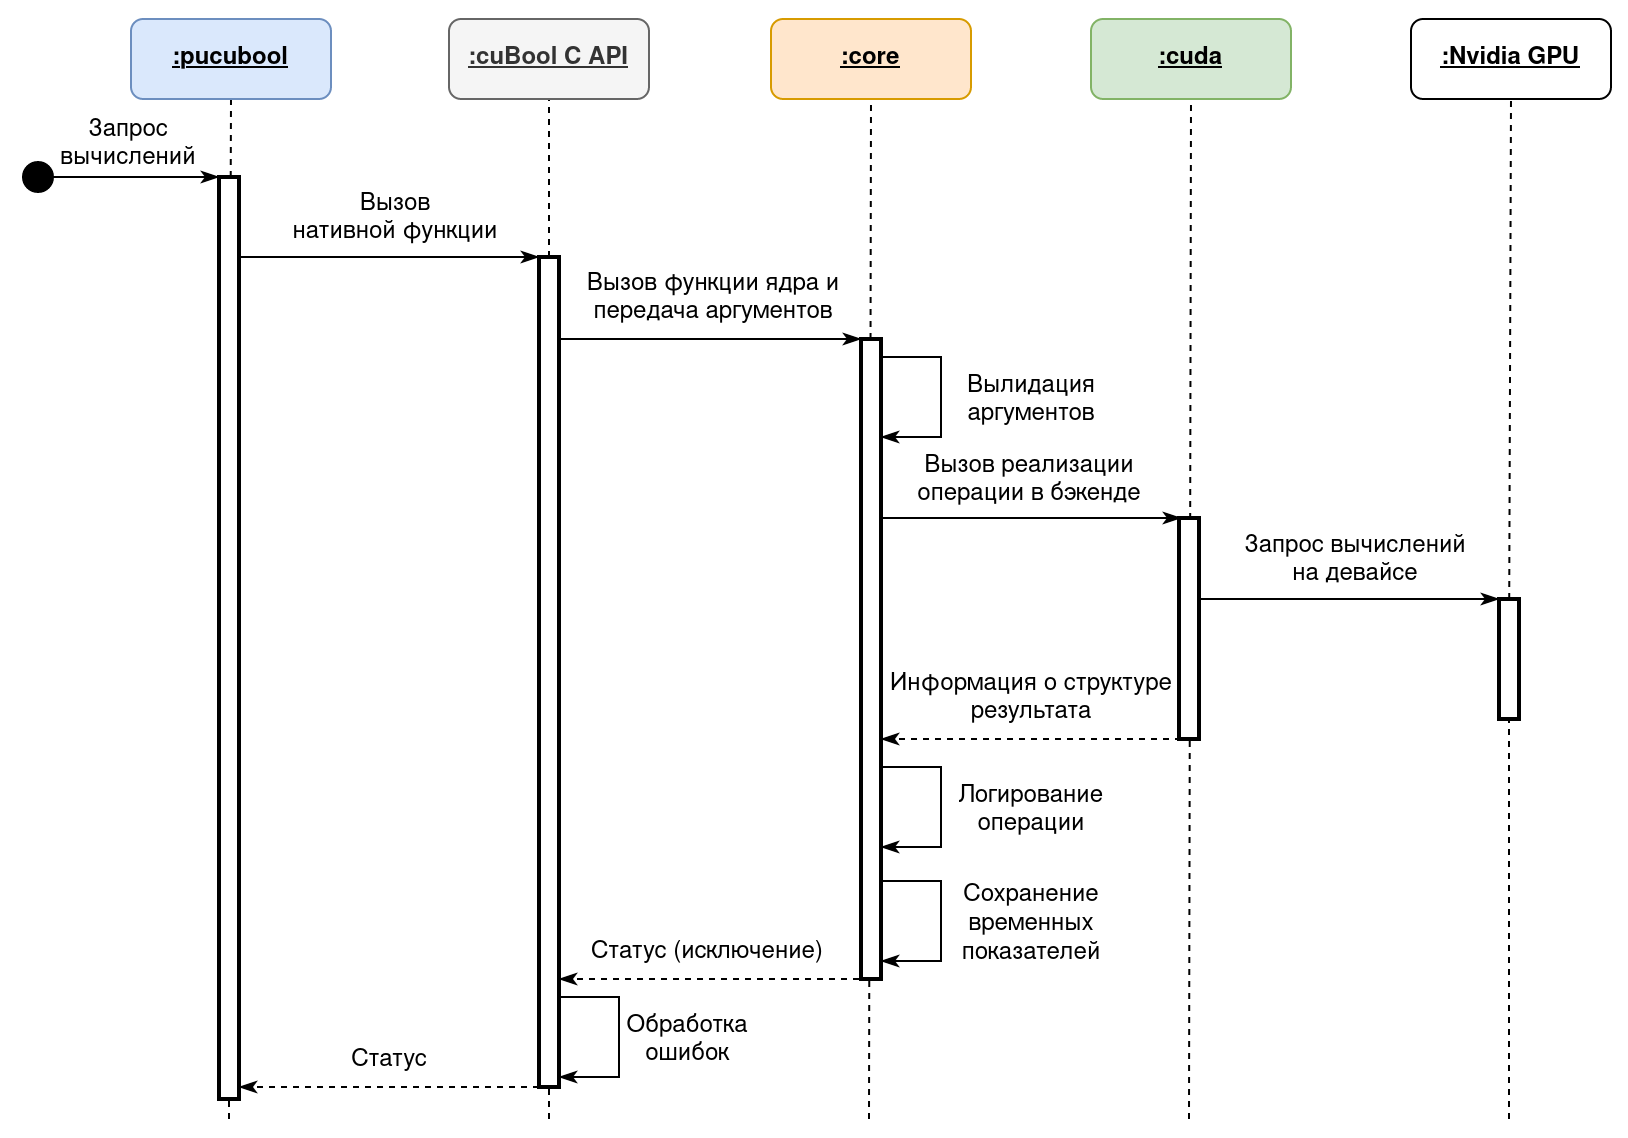
\includegraphics[width=0.9\textwidth]{images/library_sequence_use.png}
    \caption{Последовательность выполнения вычислительной матричной операции на Nvidia GPU с использованием pycubool}
    \label{fig:cubool_sequence}
\end{figure}

Пользовательский Python-код инициирует выполнение операции над матрицей или несколькими матрицами.
Этот вызов обрабатывает пакет \textbf{pycubool}, который осуществляет первичную базовую валидацию аргументов, запаковывает их и передает в нативную функцию \textbf{cuBool C API}.
На стороне реализации данного интерфейса полученные аргументы приводятся к требуемому типу и передаются далее в модуль \textbf{core}, 
который поддерживает состояние библиотеки, 
осуществляет валидацию аргументов, а также определяет допустимость выполнения операции. 
Далее вызов передается непосредственно вычислительному модулю \textbf{cuda}, 
который осуществляет подготовку и непосредственный запуск вычислений на стороне \textbf{Nvidia GPU}. 

Когда вычисления завершаются, \textbf{cuda}-модуль обновляет состояние матриц в соответствии с полученными результатами. 
Модуль \textbf{core} осуществят финальное логирование операции, 
а также сохраняет временные показатели выполнения вычислений в файл (опционально), 
и возвращает в качестве результата выполнения статус операции или возможное исключение, 
которое могло возникнуть на этапе выполнения операции. 
\textbf{cuBool C API} осуществляет финальную обработку исключения (если таковое возникло), 
и возвращает числовой идентификатор статуса операции. 

В результате выполнения операции \textbf{pucubool} уведомляет пользователя о потенциально возникших ошибках и возвращает управление из вызываемой функции. 
Обновленное состояние библиотеки находится в \textbf{core}, а состояние матриц после выполнения операций хранится на стороне \textbf{cuda}-модуля. 